% !TEX options=--shell-escape
% Thesis template by Julian Lueken

% Optimized for literature management with JabRef + BibLaTeX

% Change user settings:
%	"keep_focus": true, --> false, to remove the annoying pop ups
%	"use_biblatex": false,
%	"builder": "traditional" --> "basic", to use biber on every compilation
\documentclass[a4paper, 11pt]{report}

% Packages
%% Input encoding
\usepackage[T1]{fontenc}
\usepackage{lmodern}
%%\usepackage[utf8]{inputenc}

%% Syntax
\usepackage{ifthen}

%% Languages and symbols
\usepackage[main=english]{babel}
\usepackage{extarrows}
\usepackage{marvosym}

%% AMS packages
\usepackage{amssymb}
\usepackage{amsmath}
\usepackage{amsthm}

%% Citations and references
\usepackage[style=alphabetic, backend=biber]{biblatex} 
\usepackage[hidelinks]{hyperref}
\usepackage{csquotes}
\usepackage{nameref}
\usepackage{cleveref}
\usepackage{listings}

%% Page geometry
\usepackage[onehalfspacing]{setspace}
\usepackage[top=30mm, left=25mm, right=25mm, bottom=20mm]{geometry}
\usepackage{titlesec}

%% Figures and graphics
\usepackage{graphicx}
\usepackage{xcolor}
\usepackage{colortbl}
\usepackage{subcaption}
\usepackage{tikz}
\usepackage{float}
\usepackage{svg}

%% Pseudo-code
\usepackage{algorithm}
\usepackage[noend]{algpseudocode}

%% Testing
\usepackage{lipsum}

%% Package settings
%%% BibLaTeX resource (JabRef output file)
\addbibresource{../bibtex/bibliography.bib}

%%% Hyperref options
\hypersetup{hypertexnames=false}

%%% Listings options (for writing code in LaTeX)
\lstset{numbers=left, numberstyle=\tiny, numbersep=5pt}
\lstset{language=Python}

%%% AMS environment definitions
\theoremstyle{definition}
\newtheorem{definition}{Definition}[section]
\newtheorem{example}[definition]{Example}
\newtheorem{theorem}[definition]{Theorem}
\newtheorem{corollary}[definition]{Corollary}
\newtheorem*{remark}{Remark}
\newenvironment{myAbstract}{\section*{Abstract}}{}

%%% Special formatting
\renewcommand{\emph}[1]{\textit{#1}}
\newcommand{\mytitle}[1]{\LARGE{#1}\normalsize\\[0.3em]}
\newcommand{\titlespace}{\vspace{2em}}
\newcommand{\smallspace}{\vspace{1em}}
\newcommand{\hugespace}{\vspace{17em}}
\newcommand{\logoheight}{4em}

%% Special formatting for pesudocode
\algblock{Input}{EndInput}
\algnotext{EndInput}
\algblock{Output}{EndOutput}
\algnotext{EndOutput}
\newcommand{\Desc}[2]{\State \makebox[12em][l]{#1}#2}


\begin{document}

% Chapter format
\titleformat{\chapter}[hang]{\normalfont\huge\bfseries}{\thechapter}{0.75em}{\huge\bfseries}
\titlespacing*{\chapter}{0em}{0em}{1em}

% Title page
\pagenumbering{gobble}
\newgeometry{top=35mm, left=20mm, right=20mm, bottom=10mm}
\begin{titlepage}
	\begin{center}
		\begin{minipage}{.49\textwidth}
			\flushleft
			\includegraphics[height=\logoheight]{../assets/formal/logo_gau.png}
		\end{minipage}
		\begin{minipage}{.49\textwidth}
			\flushright
			\includegraphics[height=\logoheight]{../assets/formal/logo_dlr.png}	
		\end{minipage}
		\begin{minipage}{.49\textwidth}
			\begin{center}
				\vspace{2cm}
				Master's thesis in\\
				Applied Computer Science\\
				\titlespace
				\mytitle{CoolingGen}
				A parametric 3D-modeling software for turbine blade cooling geometries using NURBS\\
				\titlespace
				\today\\
				\hugespace
				Institute for Numerical and Applied Mathematics at the Georg-August-University Göttingen\\
				\titlespace
				Institute for Propulsion Technology at the German Aerospace Center in Göttingen\\
				\titlespace
				Bachelor's and master's theses at the Center for Computational Sciences at the Georg-August-University Göttingen\\
				\titlespace
				Julian Lüken\\
				\texttt{julian.lueken@dlr.de}\\
			\end{center}
		\end{minipage}
	\end{center}
\end{titlepage}
\pagebreak

% Address page
\pagestyle{empty}
\restoregeometry
\newgeometry{top=210mm, left=45mm, right=45mm}
\noindent
\begin{tabular}{l}
Georg-August-University Göttingen\\
Institute of Computer Science\\
\end{tabular}\\[1em]
\begin{tabular}{ll}
	\Telefon 	&+49 (551) 39-172000\\
	\FAX 		&+49 (551) 39-14403\\
	\Letter 	&\texttt{office@cs.uni-goettingen.de}\\
\end{tabular}\\[1em]
\begin{tabular}{l}
\texttt{www.informatik.uni-goettingen.de}\\
\end{tabular}\\[1em]
\pagebreak

% Done-it-myself page
\noindent I hereby declare that this thesis has been written by myself and no other resources than those mentioned have been used.\\[0.7em]
\phantom{H}\includegraphics[height=3em]{../assets/formal/sign.png}\\[0.5em]
Göttingen, \today \hspace{2em}
\pagebreak

% Abstract and Zusammenfassung
\restoregeometry
\begin{abstract}
	\thispagestyle{plain}
	\pagenumbering{roman}
	\setcounter{page}{3}
	\lipsum[1-3]
\end{abstract}
\renewcommand{\abstractname}{Zusammenfassung}
\begin{abstract}
	\thispagestyle{plain}
	\pagenumbering{roman}
	\setcounter{page}{4}
	\lipsum[4-6]
\end{abstract}
\pagebreak

% Table of contents
\setcounter{page}{5}
\restoregeometry
\tableofcontents
\pagebreak

% Actual document starts here
\restoregeometry
\pagenumbering{arabic}
\setcounter{page}{1}
\pagestyle{plain}

\chapter{Introduction}
\section{Motivation}
\section{State of the Art}
\section{Problem Statement}

\chapter{Methods}
\section{Bézier Curves}
Bézier curves are named after the French engineer Pierre Bézier, who famously utilized them in the 1960s to design car bodies for the automobile manufacturer Renault \cite{Bezier1968}. Today, they are used in a wide variety of vector graphics applications (i.e. in font representation on computers). At first glance, the definition of the Bézier curve might seem cumbersome, but given the mathematical foundation and a few graphical representations, it becomes apparent why they are such a powerful tool in computer-aided design.

\begin{figure}[!ht]
	\centering
	\begin{subfigure}{0.25\textwidth}
		\includesvg[width=\textwidth]{../python/bezierDifferentDegrees1}
		\caption{Degree $1$.}
	\end{subfigure}
	\begin{subfigure}{0.25\textwidth}
		\includesvg[width=\textwidth]{../python/bezierDifferentDegrees2}
		\caption{Degree $2$.}
	\end{subfigure}
	\begin{subfigure}{0.25\textwidth}
		\includesvg[width=\textwidth]{../python/bezierDifferentDegrees3}
		\caption{Degree $3$.}
	\end{subfigure}
	\caption{Beziér curves of different degrees (orange) and their control points (blue).}
\end{figure}

\subsection{Definition}
\begin{definition}
	The \emph{Bernstein basis polynomials} of degree $n$ on the interval $[t_0,t_1]$ are defined as
	\begin{equation}\label{eq:bernsteinbasisdef}
		b_{n,k,[t_0, t_1]}(t) := \frac{\binom{n}{k} (t_1-t)^{n-k}(t-t_0)^k}{(t_1-t_0)^n},
	\end{equation}
	for $k \in \{0,\dots, n\}$.
\end{definition}

\begin{definition}
	A \emph{Bézier curve} of degree $n$ is a parametric curve $B_{P,[t_0, t_1]}: [t_0, t_1] \rightarrow \mathbb{R}^3$ that has a representation
	\begin{equation}\label{eq:bezierdef}
		B_{P, [t_0, t_1]}(t) = \sum_{k=0}^n b_{n,k,[t_0, t_1]}(t) P_k = \sum_{k=0}^n \frac{\binom{n}{k} (t_1-t)^{n-k}(t-t_0)^k}{(t_1-t_0)^n} P_k.
	\end{equation}
	We call the elements of the set $P = \{P_0, P_1, \dots, P_n\}$ the \emph{control points} of $B_P$.
\end{definition}

\begin{remark}
	Let $t_0 = 0$ and $t_1 = 1$. Then \ref{eq:bezierdef} simplifies to
	\begin{equation}
		b_{n,k}(t) := b_{n,k,[0,1]}(t) = \binom{n}{k} (1-t)^{n-k}t^k
	\end{equation}
	and \ref{eq:bernsteinbasisdef} simplifies to
	\begin{equation}\label{eq:bezierdefshort}
		B_P(t) := B_{P,[0,1]}(t)= \sum_{k=0}^n \binom{n}{k} (1-t)^{n-k}t^k P_k.
	\end{equation}
	This case is the only case considered in this thesis.
\end{remark}

\subsection{de Casteljau's Algorithm}

The computation of equation \ref{eq:bezierdefshort} is usually performed using de Casteljau's algorithm. This is because the algorithm yields a simple implementation and lower complexity than straightforwardly computing equation \ref{eq:bezierdefshort}. The algorithm was proposed by Paul de Faget de Casteljau for the automobile manufacturer Citroën in the 1960s.

\begin{algorithm}
	\begin{algorithmic}[1]
		\Input
			\Desc{$P = \{P_0, P_1, ..., P_n\}$}{set of control points}
			\Desc{$t$}{real number}
		\EndInput
		\Output
			\Desc{$P^{(n)}_0 = B_P(t)$}{the point on the Beziér curve w.r.t. to $t$}
		\EndOutput

		\caption{de Casteljau's algorithm}\label{alg:decasteljaualgo}
		\Procedure{deCasteljau}{P, t}
			\State $P^{(0)} \gets P$
			\For {$i = 1, 2, ..., n$}
				\For {$j = 0, 1, ..., n-i$}
					\State $P^{(i)}_j \gets (1-t) \cdot P^{(i-1)}_j + t \cdot P^{(i-1)}_{j+1}$
				\EndFor
			\EndFor
			\Return $P^{(n)}_0$
		\EndProcedure
	\end{algorithmic}
\end{algorithm}

\begin{theorem}
	Algorithm \ref{alg:decasteljaualgo} computes $B_P(t)$.
\end{theorem}
\begin{proof}
	By induction. Let $n = 1$. Then
		$$ P_0^{(1)} = (1-t) \cdot P_0 + t \cdot P_1.$$
	By employing the induction hypothesis
		$$ P_j^{(n)} = \sum_{k=j}^{n+j} \binom{n}{k} (1-t)^{n-k}t^k P_{j+k}$$
	for some $n \in \mathbb{N}$, we can infer that
	\begin{align*}
		P_0^{(n+1)}	&= (1-t) \cdot P_0^{(n)} + t \cdot P_1^{(n)} \\
					&= (1-t) \cdot \sum_{k=0}^{n} \binom{n}{k} (1-t)^{n-k}t^k P_{k} + t \cdot \sum_{k=1}^{n+1} \binom{n}{k} (1-t)^{n-k}t^k P_{k+1} \\
					&= \sum_{k=0}^{n+1} \binom{n+1}{k} (1-t)^{n+1-k}t^k P_{k},
	\end{align*}
	which is equal to $B_P(t)$ for degree $n+1$.
\end{proof}

A visual representation of algorithm \ref{alg:decasteljaualgo} yields a triangular scheme. To compute one point on a Beziér curve $B_P$ with degree $n$, one has to perform $\frac{n^2-n}{2}$ additions and $n^2-n$ scalar multiplications.

\begin{figure}[!h]
	\centering
	\begin{subfigure}{0.49\textwidth}
		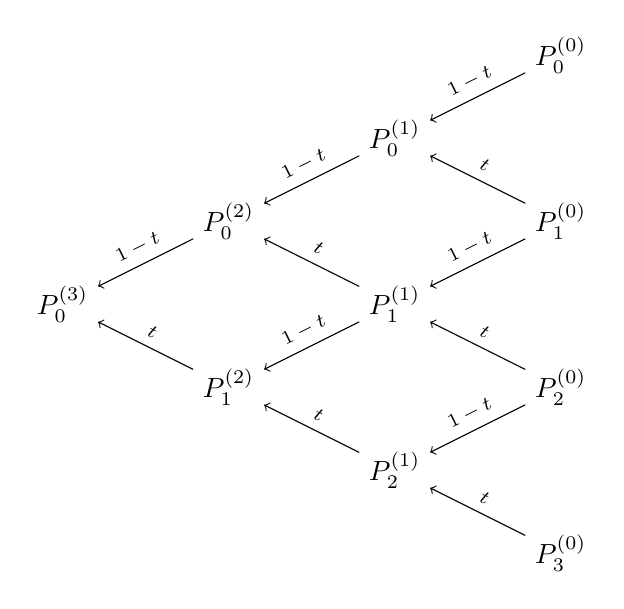
\begin{tikzpicture}
			\def\dx{60pt}
			\def\dy{30pt}

			\pgfmathsetmacro{\degree}{3}

			% Make nodes
			\newcounter{i}
			\newcounter{j}

			\node (\arabic{i}) at (0,0) {$P^{(\degree)}_0$};
			\stepcounter{i}

			\foreach \x in {1, ..., \degree} {
				\pgfmathsetmacro{\xstep}{\x-2}

				\setcounter{j}{0}
				\foreach \y in {\x, \xstep, ..., -\x} {
					\node (\arabic{i}) at (\x*\dx, \y*\dy) {$P^{(\pgfmathint{\degree-\x}\pgfmathresult)}_{\arabic{j}}$};
					\stepcounter{i}
					\stepcounter{j}
				}
			}
			
			% Make arrows
			\newcounter{z}
			\newcounter{a}
			\newcounter{b}
			\pgfmathsetmacro{\maxx}{\degree}
			\foreach \x in {1,...,\degree}{
				\foreach \y in {1,...,\x}{
					
					\setcounter{a}{\arabic{z}}
					\addtocounter{a}{\x}

					\setcounter{b}{\arabic{z}}
					\addtocounter{b}{\x}
					\stepcounter{b}
					
					\draw [<-] (\arabic{z}) -- (\arabic{a}) node[above, midway, sloped] {\scriptsize $1-t$};
					\draw [<-] (\arabic{z}) -- (\arabic{b}) node[above, midway, sloped] {\scriptsize $t$};
					
					\stepcounter{z}
				}
			}
		\end{tikzpicture}
		\caption{Algorithmic visualization.}
	\end{subfigure}
	\hfill
	\begin{subfigure}{0.49\textwidth}
		\includesvg[width=\textwidth]{../python/deCasteljauVisual}
		\caption{Geometric visualization of $B_P(\frac{3}{5})$.}
	\end{subfigure}
	\caption{Visual representations of de Casteljau's algorithm.}
	\label{fig:decasteljautriangle}
\end{figure}

Interestingly, the representation of the algorithm in Figure \ref{fig:decasteljautriangle} also gives rise to an intuitive visualization of the geometric shape of the Beziér curve $B_P$. For all $i \in \{0, ..., n\}$ and all $j \in \{0, ..., n-i\}$, the point $P^{(i+1)}_j$ is the convex combination (always w.r.t. $t$) of $P^{(i)}_j$ and $P^{(i)}_{j+1}$. Thus $P^{(i+1)}_j$ always lies on the line segment between $P^{(i)}_j$ and $P^{(i)}_{j+1}$, as can also be observed in \ref{fig:decasteljautriangle}.

\subsection{Properties}
Other than being remarkably intuitive, Beziér curves have a lot of properties which make them convenient. In computer-aided design software, most graphical user interfaces rely on the principle of letting the user interactively drag and drop the control points with a mouse, granting them control over the shape of Beziér curve. The following theorems further illustrate why this is a good idea.

\begin{theorem}
	$B_P(0) = P_0$ and $B_P(1) = P_n$.
\end{theorem}
\begin{proof}
	Explicit computation yields
		$$B_P(0) = \sum_{k=0}^n \binom{n}{k} t^k P_k = \binom{n}{0} P_0 = P_0$$
	and
		$$B_P(1) = \sum_{k=0}^n \binom{n}{k} (1-t)^{n-k} P_k = \binom{n}{n} P_n = P_n.$$
\end{proof}

\begin{theorem}
	Let $T \in \mathbb{R}^{3 \times 3}$. Then $B_{TP}(t) = TB_P(t)$ where $TP := \{TP_0, TP_1, ..., TP_n\}$.
\end{theorem}
\begin{proof}
	For all $t \in [0, 1]$ we can directly compute
		$$TB_P(t) = \sum_{k=0}^n \binom{n}{k} (1-t)^{n-k}t^k TP_k = B_{TP}(t).$$
\end{proof}

\begin{theorem}
	$B_P(t)$ lies in the convex hull of $P$ for all $t \in [0,1]$.
\end{theorem}
\begin{proof}
	By the algorithm of de Casteljau (\ref{alg:decasteljaualgo}), we know that $P^{(i)}_j = (1-t) \cdot P^{(i-1)}_j + t \cdot P^{(i-1)}_{j+1}$ for all $t \in [0, 1]$. Therefore, $P^{(i)}$ lie in the convex hull of $P^{(i-1)}$. But then $B_P(t) = P^{(n)}_0$ always lies in the convex hull of $P^{(0)} = P$ by induction.
\end{proof}

Simple as their appearance may be, Beziér curves fall short of representing some of the most common geometric shapes. Given a finite number of control points, we can never make $B_P(t)$ a circular arc, although a circle has a very simple parametric form. One of their greatest perks, the ability to describe a shape with just a handful of control points, is their greatest shortcoming at the same time. This is most likely the reason why Beziér curves are not the state of the art in technical engineering applications. However, Beziér curves certainly do provide an intuition for Non-Uniform Rational B-Splines or NURBS, which is their prevailing counterpart.

\section{Non-Uniform Rational B-Splines (NURBS)}
\subsection{Definition}
Similarly to how Beziér curves are defined on the Bernstein polynomial basis, NURBS are defined on basis functions called basis splines (or more commonly B-splines), which are recursively defined on a knot sequence $(t_m) \subset \mathbb{R}$ with $t_{k+1} \geq t_k$ for all $k \in \mathbb{N}$.

\begin{definition}
	The B-splines of degree $0$ on a knot sequence $(t_m)$ are defined as
	\begin{equation}
		N^{(t_m)}_{0,k}(t) :=
		\begin{cases}
			1 & \text{if } t \in [t_k, t_{k+1}),\\
			0 & \text{else.}
		\end{cases}
	\end{equation}
	The B-splines of higher degrees are recursively given by
	\begin{equation}
		N_{n+1,k}^{(t_m)}(t) := \omega^{(t_m)}_{n, k}(t) \, N^{(t_m)}_{n, k}(t) + (1-\omega^{(t_m)}_{n, k+1}(t)) \, N^{(t_m)}_{n, k+1}(t),
	\end{equation}
	where
	\begin{equation}
		\omega^{(t_m)}_{n,k}(t) := 
		\begin{cases}
			\frac{t-t_k}{t_{k+n} - t_k} &\text{if } t_{k+n} \neq t,\\
			0 							&\text{else.}
		\end{cases}
	\end{equation}
\end{definition}

\begin{remark}
	Instead of $N_{n,k}^{(t_m)}$ we write $N_{n,k}$ and explicitly refer to $(t_m)$ when necessary. We restrict the domain of definition of $N_{n,k}$ to $[0, 1)$ by setting $\inf t_m = 0$ and $\sup t_m = 1$.
\end{remark}

\begin{theorem}
	The B-splines of degree $n$ form a partition of unity, that is
	\begin{equation}
		\sum_{k=j-n}^j N_{n,k}(t) = 1,
	\end{equation}
	for $t \in [t_j, t_{j+1})$.
\end{theorem}
\begin{proof}
	Applying the recurrence relation for B-splines, we find that $N_{n,j}$ is a linear combination of $N_{n-1, j}$ and $N_{n-1, j+1}$, which reveals that if $N_{n, j}(t) \neq 0$ then $t \in [t_j, t_{j+n+1})$. The induction hypothesis is
	\begin{equation}
		\sum_{k=j-(n-1)}^{n-1} N_{n-1,k}(t) = 1,
	\end{equation}
	which in the case of $n=1$ is true by the definition of the B-spline. Applying the definition of $\omega_{k,l}$ we get
	\begin{align*}
		\sum_{k=j-n}^j N_{n,k}(t)	&= \sum_{k=j-n}^j \omega_{n-1, k}(t) N_{n-1, k}(t) + (1-\omega_{n-1, k+1}) N_{n-1, k+1}(t) \\
									&= \omega_{n-1, j-n}(t) N_{n-1, j-n}(t)\\
									&+ \sum_{k=j}^{n+j} \left(\frac{t_{n+k-1} - t}{t_{n+k-1} - t_{k}} + \frac{t - t_k}{t_{n+k-1} - t_k}\right) N_{n-1,k}(t)\\
									&+ \omega_{n-1, j+1}(t) N_{n-1, j+1}(t).
	\end{align*}
	For the given $t$, the B-spline $N_{n-1, j-n}(t)$ is equal to zero, because $t \in [t_j, t_{j+1})$ and $N_{n-1, j-n} \equiv 0$ except on the interval $[t_{j-n}, t_j)$.
	Similarly, $N_{n-1, j+1}(t)$ is equal to zero, because $N_{n-1, j+1} \equiv 0$ except on the interval $[t_{j+1}, t_{n+j+1})$. Therefore, the above equation is equal to
	\begin{equation}
		\sum_{k=j-n+1}^{n-1} N_{n-1,k}(t),
	\end{equation}
	which is equal to $1$ by the induction hypothesis.
\end{proof}

One of the differences of B-splines compared to the Bernstein polynomials is the local support. While for all Bernstein polynomials of degree $n$ we have $\text{supp}\;b_{n,k} = [0, 1]$, it is often the case that $\text{supp}\;N_{n,k} \subsetneq [0, 1]$. However, we do have the property that $\bigcup_k \text{supp} \; N_{n,k} = [0,1]$. This idea geometrically translates to the fact that a B-spline curve is defined for all values of $t \in [0,1]$ but shifting single control points only results in local changes, whereas in Beziér curves, a shift of a single control point is going to affect the curve globally.

In practice, the notion of the knot sequence is commonly simplified to that of a knot vector $T$, which only contains a finite number of elements. We also require a set $P$ of control points to draw curves.

\begin{definition}
	A NURBS curve $C_P(t)$ of degree $n$ with the control points $P = \{P_0, P_1, ..., P_k\}$, the control weights $W = (w_0, w_1, ... w_k)$ and a knot vector $T = (t_0, t_1, ..., t_{k+n+1})$ with the property $t_{i+1} \geq t_{i}$ for all $i \in [0, k+n]$ is defined as
	\begin{equation}
		C_P(t) = \sum_{i=0}^k R_{n,i}(t)P_i,
	\end{equation}
	where
	\begin{equation}
		R_{n,i}(t) = \frac{N_{n,i}(t)w_i}{\sum_{j=0}^k N_{n,j}(t) w_j}
	\end{equation}
	are called rational basis functions.
\end{definition}

The degree of a Beziér curve $B_P(t)$ is equal to $|P|-1$, whereas in a NURBS curve $C_P(t)$, the number of points and the degree are only related by the knot vector.

\subsection{de Boor's Algorithm}
To efficiently calculate points on a NURBS curve, Carl-Wilhelm Reinhold de Boor devised an efficient algorithm for B-splines. The common strategy that utilizes this algorithm for NURBS curves employs the following steps. Using the map 
	$$\Phi: \{P, W\} \mapsto P^W$$
we can construct the set of weighted control points $P^W$, where $P^W_i = (w_i P_{i_x}, w_i P_{i_y}, w_i P_{i_z}, w_i)$. We can then use de Boor's algorithm to calculate the weighted B-spline curve $C^W$ on the set of weighted control points. Afterwards, we use the perspective map 
	$$\Phi^\dagger: C^W \mapsto C$$ 
to retrieve the NURBS curve $C$.



\begin{algorithm}
	\begin{algorithmic}[1]
		\Input
			\Desc{$P = \{P_0, P_1, ..., P_k\}$}{set of control points of the NURBS curve}
			\Desc{$W = \{w_0, w_1, ..., w_k\}$}{weights of the control points}
			\Desc{$T = (t_0, t_1, ..., t_{k+n+1})$}{knot vector of the NURBS curve}
			\Desc{$n$}{degree of the NURBS curve}
			\Desc{$t \in [t_0, t_{k+n+1})$}{real number}
		\EndInput
		\Output
			\Desc{$C_P(t)$}{the point on the NURBS curve w.r.t. to $t$}
		\EndOutput

		\caption{de Boor's algorithm}\label{alg:debooralgo}
		\Procedure{deBoor}{P, p, T, t}
			\State $P^{(0)} \gets \Phi(P, W)$
			\State Find $l$ such that $t \in [t_l, t_{l+1})$
			\State Let $m$ be the multiplicity of $t$ in the knot vector $T$

			\For {$i = 1, 2, ..., n-m$}
				\For {$j = l-n+i, ..., l-m$}
					\State $\alpha^{(i)}_j \gets \frac{t-t_j}{t_{j+n-i+1} - t_j}$
					\State $P^{(i)}_j \gets (1-\alpha^{(i)}_j) \cdot P^{(i-1)}_ {j-1} + \alpha^{(i)}_j \cdot P^{(i-1)}_j$
				\EndFor
			\EndFor

			\Return $\Phi^\dagger(P^{(n-m)}_{l-m}) = C_P(t)$
		\EndProcedure
	\end{algorithmic}
\end{algorithm}

De Boor's algorithm is a generalization of de Castlejau's algorithm. 

\begin{figure}[h!]
	\centering
	\begin{tikzpicture}
		\def\dx{90pt}
		\def\dy{30pt}

		\pgfmathsetmacro{\degree}{3}

		% Make nodes
		\setcounter{i}{0}
		\setcounter{j}{0}

		\node (\arabic{i}) at (0,0) {$P^{(\degree)}_l$};
		\stepcounter{i}

		\foreach \x in {1, ..., \degree} {
			\pgfmathsetmacro{\xstep}{\x-2}

			\setcounter{j}{0}
			\foreach \y in {\x, \xstep, ..., -\x} {

				\ifthenelse{\value{j}>0} {
					\node (\arabic{i}) at (\x*\dx, \y*\dy) {$P^{(\pgfmathint{\degree-\x}\pgfmathresult)}_{l-\arabic{j}}$};
				}
				{
					\node (\arabic{i}) at (\x*\dx, \y*\dy) {$P^{(\pgfmathint{\degree-\x}\pgfmathresult)}_l$};
				}
				\stepcounter{i}
				\stepcounter{j}
			}
		}
		
		% Make arrows
		\setcounter{z}{0}
		\setcounter{a}{0}
		\setcounter{b}{0}
		\pgfmathsetmacro{\maxx}{\degree}
		\foreach \x in {1,...,\degree}{
			\foreach \y in {1,...,\x}{
				
				\setcounter{a}{\arabic{z}}
				\addtocounter{a}{\x}

				\setcounter{b}{\arabic{z}}
				\addtocounter{b}{\x}
				\stepcounter{b}
				
				\ifthenelse{\y > 1} {
					\draw [<-] (\arabic{z}) -- (\arabic{b}) node[above, midway, sloped] {\scriptsize $1-\alpha^{(\pgfmathint{\degree-\x+1}\pgfmathresult)}_{l-\pgfmathint{\y-1}\pgfmathresult}$};
					\draw [<-] (\arabic{z}) -- (\arabic{a}) node[above, midway, sloped] {\scriptsize $\alpha^{(\pgfmathint{\degree-\x+1}\pgfmathresult)}_{l-\pgfmathint{\y-1}\pgfmathresult}$};
				}
				{
					\draw [<-] (\arabic{z}) -- (\arabic{b}) node[above, midway, sloped] {\scriptsize $1-\alpha^{(\pgfmathint{\degree-\x+1}\pgfmathresult)}_l$};
					\draw [<-] (\arabic{z}) -- (\arabic{a}) node[above, midway, sloped] {\scriptsize $\alpha^{(\pgfmathint{\degree-\x+1}\pgfmathresult)}_l$};
				}

				\stepcounter{z}
			}
		}
	\end{tikzpicture}
	\caption{Algorithmic visualization.}
\end{figure}

\begin{theorem}
	Algo works
\end{theorem}
\begin{proof}
	By induction. Let $n = 1$ and $t \in (t_l, t_{l+1})$. Then
	\begin{align*}
		P_l^{1} &= (1-\alpha_l^{(1)}) \cdot P_{l-1}^{(0)} + \alpha_l^{(1)} \cdot P_l^{(0)} \\
				&= \left(1-\frac{t-t_l}{t_{l+1}-t_l}\right) \cdot P_{l-1}^{(0)} + \frac{t-t_l}{t_{l+1}-t_l} \cdot P_l^{(0)} \\
				&= (1-\omega_{1,l}) \cdot (w_{l-1} P_{l-1}, w_{l-1}) + \omega_{1,l} \cdot (w_l P_l, w_l) \\
				&= N_2
	\end{align*}
	Applying the perspective map $\Phi^\dagger$, we find that this is equal to $C_P(t)$.

	\begin{align*}
		P^{(n)}_l 	&= (1-\alpha_l^{(n)}) \cdot P_{l-1}^{(n-1)} + \alpha_l^{(n)} \cdot P_l^{(n-1)} \\
					&= 
	\end{align*}

\end{proof}


\subsection{Properties}


\section{Methods on NURBS Objects}
\subsection{Affine Transformations}
\subsection{The Frenet-Serret Apparatus}
\subsection{Finding Intersections}
\subsection{Interpolation}

\section{Jet Engine Design Specifics}
\subsection{Fundamental Terms}
\subsection{The S2M Net}
\subsection{Fillet Creation}
\begin{figure}[!ht]
	\centering
	\includesvg[width=0.5\textwidth]{../python/filletVisuals}
	\caption{yeah}
\end{figure}

\chapter{Results}
\section{Cooling Geometries And Their Parametrizations}
\subsection{Chambers}
\subsection{Turnarounds}
\subsection{Slots}
\subsection{Film Cooling Holes}
\begin{figure}[!ht]
	\centering
	\includesvg[width=0.5\textwidth]{../python/fanshapedCurveDefinition}
	\caption{yeah}
\end{figure}
\begin{figure}[!ht]
	\centering
	\includesvg[width=0.5\textwidth]{../assets/tecplot/selfIntersection}
	\caption{yeah}
\end{figure}


\subsection{Impingement Inserts}
\section{Export for CENTAUR}
\section{Export for Open CASCADE}

\chapter{Discussion}
\section{Future Work}
\section{Conclusion}
\cite{Piegl1997}

% Bibliography, numbered and formatted like a chapter (for the TOC as well)
\printbibliography[heading=bibnumbered, title=References]

\end{document}